
\section{ソフトの構成と描画}
\subsection{外部データの読み込み部}
\subsubsection{read\_pos}\begin{quote}\begin{verbatim}
def read_pos(lines, init_line=8)
  lattice, atom, poscar = [],[],[]
  lines[2..4].each{|line| lattice << line.scanf("%f %f %f\n")  }

  lines[init_line..lines.length+1].each{|line| atom << line.scanf("%f %f %f\n") }

  atom.each{|i_atom|
    pos=[0.0,0.0,0.0,0.0]
    i_atom.each_with_index{|atom_j,j|
      lx,ly,lz=lattice[j]
      pos[0] += atom_j*lx
      pos[1] += atom_j*ly
      pos[2] += atom_j*lz
    }
    poscar << pos
  }
  return poscar
end
\end{verbatim}\end{quote}
外部データであるPOSCAR\_2223をARGVで読み込み,linesとして定義している.
linesの2行目から4行目の値を読み込んで,配列lattticeに格納している.
linesの8行目から最後の行の値を読み込んで,配列atomsに格納している.
配列lattice内に格納された各々の座標をlx,lylzと定義し,格子の座標と原子の座標を掛け算して粒界配列の座標を出し,その値をposcarに格納している.\verb|{{br}}|
poscarに格納された原子座標が以下の実行結果である.
\begin{quote}\begin{verbatim}
[Narita-no-MacBook-Air:~/boundary/narita/view] nari% ruby final.rb POSCAR_2223 POSCAR_2223_4
[5.75101295815, 0.0, 0.0, 0.0]
[7.668017277916733, 0.6390014395849836, 2.020699977875, 0.0]
[3.834008638383265, 0.6390014395849836, 2.020699977875, 0.0]
[7.029015837611088, 2.556005758968566, 0.0, 0.0]
[4.473010078688911, 2.556005758968566, 0.0, 0.0]
[5.75101295815, 0.0, 4.04139995575, 0.0]
[7.668017277916733, 0.6390014395849836, 6.062099933625, 0.0]
[3.834008638383265, 0.6390014395849836, 6.062099933625, 0.0]
[7.029015837611088, 2.556005758968566, 4.04139995575, 0.0]
[4.473010078688911, 2.556005758968566, 4.04139995575, 0.0]
[6.390014398455645, 4.473010078352149, 2.020699977875, 0.0]
[5.112011517844354, 4.473010078352149, 2.020699977875, 0.0]
[6.390014398455645, 4.473010078352149, 6.062099933625, 0.0]
[5.112011517844354, 4.473010078352149, 6.062099933625, 0.0]
...
[1.2780028794610885, 5.751012958150748, 6.062099933625, 0.0]
\end{verbatim}\end{quote}
\subsection{原子座標の計算部}
\subsubsection{identical\_atoms}\begin{quote}\begin{verbatim}
def identical_atom(i_atom,j_atom)
  dist=0.0
  3.times{|i| dist += (i_atom[i]-j_atom[i])**2  }
  return true if Math.sqrt(dist)<0.5
  return false
end
\end{verbatim}\end{quote}
関数identical\_atomsは,2つのPOSCARファイルに含まれる各々の原子座標の距離を求めて,ある値の大小比較をおこなって真偽を判定する機能を果たしている.
具体的には,ファイル内のある原子i\_atomともう片方のファイル内にある原子j\_atomの距離が0.5より小さい値であればtrueと判定して返す.
そうでなければ,falseを返して終了する.

\subsubsection{mk\_deleted\_atom}\begin{quote}\begin{verbatim}
def mk_deleted_atom
  mark=[]
  j_max = $pos_after.length
  $pos_before.each_with_index{|i_atom,i|
    update_num=0
    $pos_after.each_with_index{|j_atom,j|
      break if identical_atom(i_atom,j_atom)
      update_num = j
    }
    mark << $pos_before[i] if update_num==(j_max-1)
  }
  return mark
end
\end{verbatim}\end{quote}
関数mk\_deleted\_atomは,原子削除をおこなう前後のPOSCARファイルを比較して削除された原子のみを別の配列に格納する機能を果たしている.
関数内では,始めに更新するための値update\_numを0と定め,2つのPOSCARファイルをeach文で繰り返しながら,identical\_atomでtrueとして返されたものを配列markの方へ
格納している.\verb|{{br}}|
原子座標ファイルPOSCAR\_2223において,配列markに格納された原子座標が以下の実行結果である.
\begin{quote}\begin{verbatim}
[Narita-no-MacBook-Air:~/boundary/narita/view] nari% ruby final.rb POSCAR_2223 POSCAR_2223_4
[[6.390014398455645, 4.473010078352149, 2.020699977875, 0.0] 
[5.112011517844354, 4.473010078352149, 6.062099933625, 0.0] 
[10.863024475994353, 3.8340086387671652, 0.0, 0.0]
 [0.6390014403056455, 3.8340086387671652, 0.0, 0.0] 
[10.863024475994353, 3.8340086387671652, 4.04139995575, 0.0]]
\end{verbatim}\end{quote}
\subsection{粒界原子の描画部}
\subsubsection{draw\_backcolor, draw\_exes}\begin{quote}\begin{verbatim}
def draw_backcolor
  $context.set_source_rgb(0.8, 0.8, 0.8)
  $context.rectangle(0, 0, $width, $height)
  $context.fill
end

def draw_axes
  $context.set_source_rgb(0, 0, 0)
  [[0,1],[1,0]].each{|line|
    x,y=line[0],line[1]
    [[0,0],[$cx,0],[0,$cy]].each{|c_x,c_y|
      $context.move_to($mv+c_x,$mv+c_y)
      $context.line_to($mv+c_x+x*$scale,$mv+c_y+y*$scale)
      $context.stroke
    }
  }
end
\end{verbatim}\end{quote}
関数draw\_backcolorは,原子配列の背景を描画しており,SVGで表示する画面のサイズを明確にするために作成している.
また,関数draw\_axesは,原子配列における縦軸と横軸を描画しており,each文で3つ平面に必要な軸をまとめて出力できるようにしている.

\subsubsection{open\_circle}
\subsubsection{draw\_each\_plane, pos\_y}\begin{quote}\begin{verbatim}

def draw_each_plane(ind_1,ind_2,c_x,c_y)
  rr = 2
  layer_num = 3
  sel = (ind_1==0 and ind_2==1)? 1 : 0
    [[$deleted_atoms,[1,0,0],rr*1.3],[$pos_after,[0,0,1],rr]].each{|atoms_color|
    $context.set_source_rgb(atoms_color[1])
    radius = atoms_color[2]
    atoms_color[0].each{|pos|
      if open_circle[layer_num-1] < pos[2] && pos[2] < open_circle[layer_num] then
        $context.circle($mv+c_x+$adjust*pos[ind_1],pos_y(pos,c_y,ind_2,sel), radius*1.7)
        $context.stroke
        $context.set_line_width(0.5)
      else
        $context.circle($mv+c_x+$adjust*pos[ind_1],pos_y(pos,c_y,ind_2,sel), radius)
        $context.fill
      end
    }
  }

  if $pos_before.size==$pos_after.size
    $context.set_source_rgb(0, 0.8, 0)
    (0..$pos_before.length-1).each{|i|
      $context.move_to($mv+c_x+$adjust*$pos_before[i][ind_1],pos_y($pos_before[i],c_y,ind_2,sel))
      $context.line_to($mv+c_x+$adjust*$pos_after[i][ind_1],pos_y($pos_after[i],c_y,ind_2,sel))
      $context.stroke
    }
  end
end

def pos_y(pos, c_y, index, select)
  dy = select == 0 ? pos[index] : $pos_max[index]-pos[index]
  return $mv+c_y+$adjust*dy
end
\end{verbatim}\end{quote}
関数draw\_each\_planeで,描画する原子の位置,色,大きさを定めており,関数pos\_yはx−y平面でのy軸を逆転する計算をおこなっている.
具体的に,selで描画する平面の判定をおこない,x−y平面ならば,関数pos\_yで一番大きいy座標の値から各y座標を差分した値を受け取っている.
layer\_numは,白抜きするz層を指定しており,関数open\_circleをもとに白抜きする原子を判定している.
また,読み込んだ2つの原子配列ファイルPOSCARのデータサイズが同じならば,各原子の位置に相当する原子との距離を線で表示する.

\subsubsection{draw\_atoms}\begin{quote}\begin{verbatim}
def draw_atoms
  draw_each_plane(0,1,0,0)    
  draw_each_plane(0,2,0,$cy)   
  draw_each_plane(1,2,$cx,$cy) 
end
\end{verbatim}\end{quote}
関数draw\_atomsでは,前の関数draw\_each\_planeで設定した原子を三面図の規定位置にそれぞれ描画するようにしている.
具体的には,x−y平面を平面図,x−z平面を正面図,y−z平面を側面図として三面図を構成させている.

\subsubsection{find\_max}\begin{quote}\begin{verbatim}
def find_max(pos)
  max = [0,0,0]
  [0,1,2].each{|ind|
    pos.length.times {|i| max[ind] = pos[i][ind] if max[ind] < pos[i][ind] }
  }
  return max
end
\end{verbatim}\end{quote}
関数find\_maxは,原子の各座標の最大値を探索する機能を果たしている.
配列posには,関数read\_posで(x,y,z)=(0,1,2)としてそれぞれの値を読み込んでおり,隣接する値の大小比較をおこなって,各座標の最大値を配列maxに格納している.

\subsubsection{main\_draw}\begin{quote}\begin{verbatim}
def main_draw(file1,file2,   model_scale = 10)
  lines1 = File.readlines(file1)
  lines2 = File.readlines(file2)
  $pos_before = read_pos(lines1,8)
  $pos_after = read_pos(lines2,8)
  $deleted_atoms = mk_deleted_atom

   $pos_max=find_max($pos_before)
   $pos_max[0].ceil*10
  $width,$height = 300,200
  $cx,$cy = $width/2.0,$height/2.0
  $mv = 10
  $scale = 1000
  $adjust = $scale/($pos_max[0].ceil*model_scale)
  surface = Cairo::SVGSurface.new('view.svg', $width, $height)
  $context = Cairo::Context.new(surface)
  $context.set_line_width($line_width)

  draw_backcolor
  draw_axes
  draw_atoms
  surface.finish
end
\end{verbatim}\end{quote}
関数main\_drawは,読み込んだ外部ファイルをlinesとして格納し,関数read\_posでつくった原子座標poscarをファイルごとに分類している.
また,rcairoで描画処理の基本となるサーフェスとコンテキストを作成し,出力場所及び出力先の形式を定めている.

\subsection{三面図による描画}
三面図は,立体を正面図,平面図,側面図の三方向からみて投影した図を展開したもので,立体の形状を2次元上で適切に表示することが出来る.
三方向から描く各図の位置は厳密に決められており,正面図を物体の最も代表的な面とし,正面図の真上に平面図,正面図の真横に側面図を描く[7].
実際に,三面図を使用して表示したPOSCAR\_2223の成功例と失敗例は図のようになる.

\begin{figure}[htbp]\begin{center}
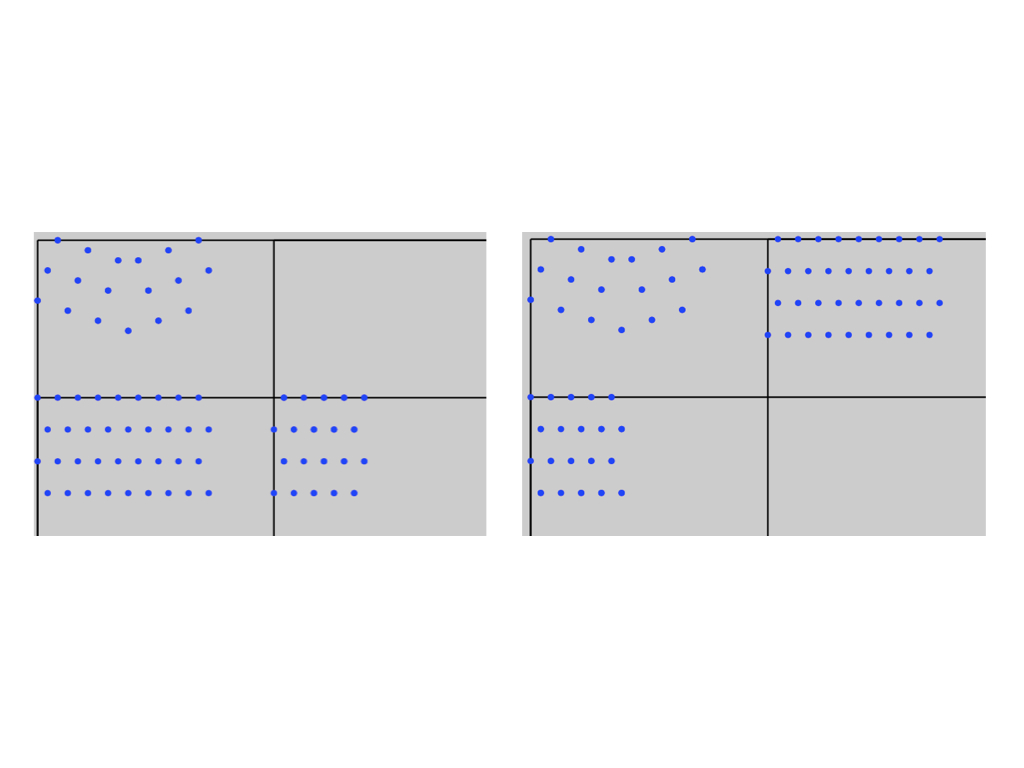
\includegraphics[width=6cm,bb=0 0 442 500]{../figs/./boundary_narita.014.jpg}
\caption{POSCAR\_2223を表示した三面図の成功例(左)と失敗例(右).}
\label{default}\end{center}\end{figure}
